\documentclass[12pt]{article}
\usepackage[margin=1in]{geometry} 
\usepackage{amsmath,amsthm,amssymb,amsfonts}
\usepackage{placeins}
\usepackage{mathtools, eucal}
 

 
\begin{document}
 
%\renewcommand{\qedsymbol}{\filledbox}
%Good resources for looking up how to do stuff:
%Binary operators: http://www.access2science.com/latex/Binary.html
%General help: http://en.wikibooks.org/wiki/LaTeX/Mathematics
%Or just google stuff
 
\title{Exam 1 Solutions}
\author{Zheming Gao}
\maketitle

\section*{Problem 1}

\begin{enumerate}
\item [(a)]

False. Counterexample:

$S_1 = \{ x = (x_1, x_2) \in \mathbb R^2 | x_2 = 0, x_1 \geqslant 0\}$ and $S_2 = \{ x = (x_1, x_2) \in \mathbb R^2 | x_1 = 0, x_2 \geqslant 0\}$.

Both $S_1$ and $S_2$ are convex but $S_1 \cup S_2$ is not convex.

\item[(b)]

True. int$(S)$ is open and the interior of an open set is itself.

\item [(c)]

False. Counterexample:

Let $P = \mathbb R_+^2$, i.e. the first quadrant. It is a unbounded polyhedron, but it is not affine. 

\item[(d)]

False. We have shown in homework that $P$ is a convex set. So if it has two points, then any convex combination of them will be in $P$.

\item[(e)]

True. The objective function $c^Tx$ is countinuous on $P$, which is a nonempty closed convex set. So $P$ is a nonempty compact set and $c^Tx$ will reach its maximum and minimum. This is supported by Weierstrass theorem.

\item[(f)]

True. We may reform $P$ as a subset on $\mathbb R^2$. So the LP problem will have one equality constraint on $\mathbb R^2$ with nonnegativeness. Hence, it has at most two positive BFS.

\item[(g)]

True. If $x$ is an optimal solution, it must be a BFS, so its nonbasic variables must be zeros. Since it has $n-m$ nonbasic variables, it has at least $n-m$ zero entries. Thus, it has at most m positive components.

\item [(h)]

False. A BS has $n-m$ nonbasic variables so it has at least $n-m$ zeros components.



\end{enumerate}

\section*{Problem 2}

\begin{enumerate}

\item[(a)]

The problem can be reformed as the following,

$$
\begin{aligned}
\text{Minimize} \quad & -x_1-x_2 \\
\text{Subject to} \quad & x_1 - x_2 \leqslant 3 \\
& x_1 - x_2 \geqslant -1\\
& x_1, x_2 \geqslant 0. 
\end{aligned}
$$

We plot the figure.

\begin{figure}[htbp]
  \caption{Problem 2}
  \centering
    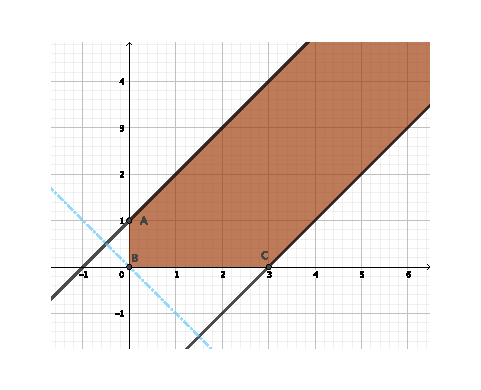
\includegraphics[width=0.5\textwidth]{p2.pdf}
\end{figure}

\FloatBarrier

From the figure we see that the problem is unbounded. This is to say that the objective value will goes to $-\infty$.

\item[(b)]

There are 5 BS, 3 BFS(with '*').

$$
\begin{aligned}
[-1, 0, 4, 0]^T \\
[3, 0, 0, 4]^T \ *\\
[0, 1, 4, 0]^T \ *\\
[0, -3, 0, 4]^T \\
[0, 0, 3, 1]^T \ * 
\end{aligned}
$$



\item[(c)]

Start from BFS $x = [0, 1, 4, 0]^T $. The basic matrix is $B = \begin{bmatrix}
A2 & A_3 
\end{bmatrix} = \begin{bmatrix}
-1 & 1 \\
-1 & 0 
\end{bmatrix}$ and so $B  = \begin{bmatrix}
0 & -1 \\
1 & -1 
\end{bmatrix}$. Hence the fundamental matrix 

$$
M = \begin{bmatrix}
-1 & 1 & 1 & 0 \\
-1 & 0 & 1 & -1 \\
0 & 0 & 1 & 0 \\
0 & 0 & 0 & 1
\end{bmatrix} \qquad M^{-1} = \begin{bmatrix}
0 & -1 & 1 & -1 \\
1 & -1 & 0 & -1 \\
0 & 0 & 1 & 0 \\
0 & 0 & 0 & 1
\end{bmatrix}.
$$

Compute reduced cost 
$$
r_1 = c^T\textbf d^1 = [-1, 0, -1, 0]\begin{bmatrix}
1\\0\\1\\0
\end{bmatrix} = -2 < 0, \quad r_2= c^T\textbf d^4 = [-1, 0, -1, 0]\begin{bmatrix}
-1\\-1\\0\\1
\end{bmatrix} = 1 > 0.
$$

Hence we take $\textbf d^1$. However, since $\textbf d^1 > 0$ and $[B|N]d = 0$ (this is easy to check). This is to say that $\textbf d^1$ is a extremal direction. Thus, $\forall \alpha > 0$ and $x + \alpha \textbf d^1$ is feasible and $c^T(x + \alpha \textbf d^1)\rightarrow -\infty$, as $\alpha \rightarrow +\infty$. Hence, the LP problem is unbounded.

\end{enumerate}

\section*{Problem 3}




\end{document}